\chapter{Methods}\label{chapter:method}

\begin{figure}[h!]
    \centering
    \includegraphics[width=0.7\textwidth]{thesis_latex_template/pics/examples_datasets.png}
    \caption[Example Images Watermark and Pattern Scenario]{First row: images from the original dSprites dataset. 
    second row: images from the watermark dataset with small \textit{w} as a watermark on some images in random positions at the edge of the image and Gaussian background noise added. 
    third row: images from the pattern dataset with either sharp or blurred noisy patterns and Gaussian background noise added.}
    \label{fig:dsprites_examples}
\end{figure}

This chapter lays out the steps necessary in our experiment to evaluate the fidelity of CRP's explanations in terms of spurious feature importance. 
After defining a causal model of the data and explanation generation process we construct the metrics we test both to yield a ground truth feature importance as well as the importance attributed in the explanation. We also describe how the experiment is conducted and through which analysis methods we compare the metrics.

\section{Benchmark Dataset}

\subsection{Watermark Scenario}\label{section:dataset_wdsprites}
Like other work using datasets with known features, we adapt an existing artificial dataset which is as simple as possible and yet mirrors the main workings of a realistic computer vision problem. For this, we alter the dSprites dataset \citep{dsprites17} by adding small watermarks in the shape of \textit{w}s to some images. The dSprites dataset was originally constructed as a means for testing the degree of disentanglement a machine learning model has achieved. It contains circa 700k images with rectangles, ellipses or hearts in varying positions, scales and rotations. To simplify the task more, we only use the rectangle and ellipse class for our experiment. Another motive is that in a binary classification task positive and negative relevance might be used in varying strategies for prediction. In theory this could make the class-insensitivity studied by \citet{Sixt2020} visible. Further details on our dataset can be found in \cref{appendix:dsprites}.

\subsection{Pattern Scenario}\label{section:dataset_overlap}
In addition to the first benchmark dataset, we deemed it necessary to conduct our experiments on a second type of problem.
The case where a spurious feature is spatially separated from the target feature has been addressed quite often and successfully with local attribution methods. Yet, in the case where features are overlapping it is not even clear how an attribution map should react ideally and how to measure the feature importance for spurious features. To analyze this case, we have created another dataset in which the pattern inside of the shape is biased. The data-generating as well as the explanation-generating model and all other parameters stay exactly the same as in the first experiment.
Images, where the spurious feature $W$, which was the watermark in the first scenario, takes the value $W=0$, have a noisy shape. If $W= 1$, instead, the pattern of the shape is blurry as seen in row three of \cref{fig:dsprites_examples}. 
For better intuition we will mostly reference the first case, where the spurious feature is a separable watermark, when laying out the next steps. Nonetheless, the measures are also applied in the same way to the pattern scenario. 

\section{Causal Model}\label{section:causal_model}
The core aspect of our analysis is the combination of causal methods for data generation and ground-truth feature attribution. 
The main process includes a hyperparameter, the later discussed coupling ratio $\rho$, which one can intervene on, together with predictions and explanations generated for multiple trained instances of a model and its output. 
Within this greater structure, a subprocess constructs the image dataset with a structural causal model taking only $\rho$ as an input. While $\rho$ stays fixed for each model to be trained, it is a causal variable in the overarching structure. This way we create an array of causally generated datasets whose constitution only differs by this one variable. 

\subsection{Data Generating Structural Causal Model}\label{section:data_gen_causal_model}
For the most exact comparison of attribution between a model and its explanation it is imperative to know the ground truth of the training data. A structural causal model (SCM) can define variables and the independent mechanisms with which they interact precisely. We want to define an SCM that closely mirrors image generation processes as they happen in realistic scenarios. 

\begin{figure}[t!]
    \centering
    \tikzset{%
        neuron/.style={
            ellipse,
            draw,
            minimum height=8mm,
            minimum width=30mm,
            inner sep=1pt,
            align=center,
            },
        arrows={[scale=1.2]}
    }
    \begin{tikzpicture}[]
    % generating model:
        \node [neuron, dashed]  (nw) at (0,4) {Watermark Noise \\$N_w$};
        \node [neuron]  (g) at (0,2) {Generator \\$G$};
        \node [neuron, dashed]  (ns) at (0,0) {Shape Noise \\$N_s$};
        \node [neuron]  (w) at (4,3) {Watermark \\$W$};
        \node [neuron]  (s) at (4,1) {Shape \\$S$};
        \node [neuron]  (x) at (8,2) {Image \\$X$};
        \node [neuron]  (z) at (8,0) {Other Factors \\$Z$};
        \node [neuron, dashed]  (nx) at (8,4) {Image Noise \\$N_x$};
        
        \draw[->] (nw) -- (w);
        \draw[->] (g) -- (w);
        \draw[->] (ns) -- (s);
        \draw[->] (g) -- (s);
        \draw[->] (s) -- (x);
        \draw[->] (w) -- (x);
        \draw[->] (z) -- (x);
        \draw[->] (nx) -- (x);
        
    \end{tikzpicture}
    \caption[Data Generating Structural Causal Model]{Data Generating Structural causal model.
        $\rho$ is not visible in the SCM. It determines the signal-to-noise ratio between the confounding $G$ and the noise variables $N_w$ and $N_s$ in the structural assignments. The noise terms of $Z$ and $G$ are not shown explicitly because they have no further causal parents.}
    \label{fig:generating_scm}
\end{figure}

The causal graph and its structural assignments used for our experiment are defined as follows: 
\begin{equation}
\label{eq:scm}
\begin{aligned}[c]
G&:=\eta^g \notag \\ 
N_w&:=\eta^w  \notag \\ 
N_s&:=\eta^s \notag \\ 
N_x&:=\eta^x  \notag \\ 
W&:=(\rho * G + (1-\rho)* N_w) \geq 0.5 \notag \\ 
S&:=(\rho * G + (1-\rho)* N_s) \geq 0.5 \notag \\ 
Z&:= \eta^z \\ 
X&:= W + f_{image}(S, Z) + N_{x} \\
\end{aligned}
\begin{aligned}[c]
& \mathrm{with} \  \eta^g \sim \mathcal{N}(0.5,0.02) && \notag \\ 
& \mathrm{with} \  \eta^w \sim \mathcal{N}(0.5,0.1) && \notag \\ 
& \mathrm{with} \  \eta^s \sim \mathcal{N}(0.5,0.1) && \notag \\ 
& \mathrm{with} \  \eta^x \sim \mathcal{N}(0,0.05) && \notag \\ 
\\
\\
& \mathrm{with} \  \eta^z \sim \mathcal{U}(0,245760) && \notag \\ 
\\
\end{aligned}
\end{equation}

These assignments are visualized in the causal graph in \cref{fig:generating_scm}.
Variables of interest are the spurious (watermark) feature $W$ and the target (shape) feature $S$ as well as their combination, the image variable $X$. $N$ represent noise or unobserved variables, $G$ the generator confounding $S$ and $W$, and $Z$ a multivariate variable describing all other factors of the dataset. 

The SCM, as seen in \cref{fig:generating_scm} and \cref{eq:scm}, serves as a ground truth for our experiment. It is mostly an additive model using Gaussian distributions for the noise terms, except for $Z$ which uniformly selects other image generating factors like rotation, scale and position of a shape. Further, the function $f_{image}$ generating the images out of the latent factors and the shape is not further specified.

The meta-variable $\rho$ adjusts how much information is shared between the true class information \textit{is shape} or target feature and the \textit{has watermark} information or spurious feature through a shared common ancestor named \textit{generator} $G$. For each model, coupling ratio $\rho$ is fixed to later enable a comparison between models trained with different coupling ratios. 
A second parameter which we keep fixed for all experiments, determines how frequent the spurious feature is in the data. We set this parameter which can be seen as the \textit{prevalence} to one half, so that just as many images have a watermark as not. Notably, when $\rho$ is one this means that all ellipses will have the watermark and no rectangle will and when $\rho$ is zero there is no correlation of watermark and shape. 

\begin{figure}[t!]
    \centering
    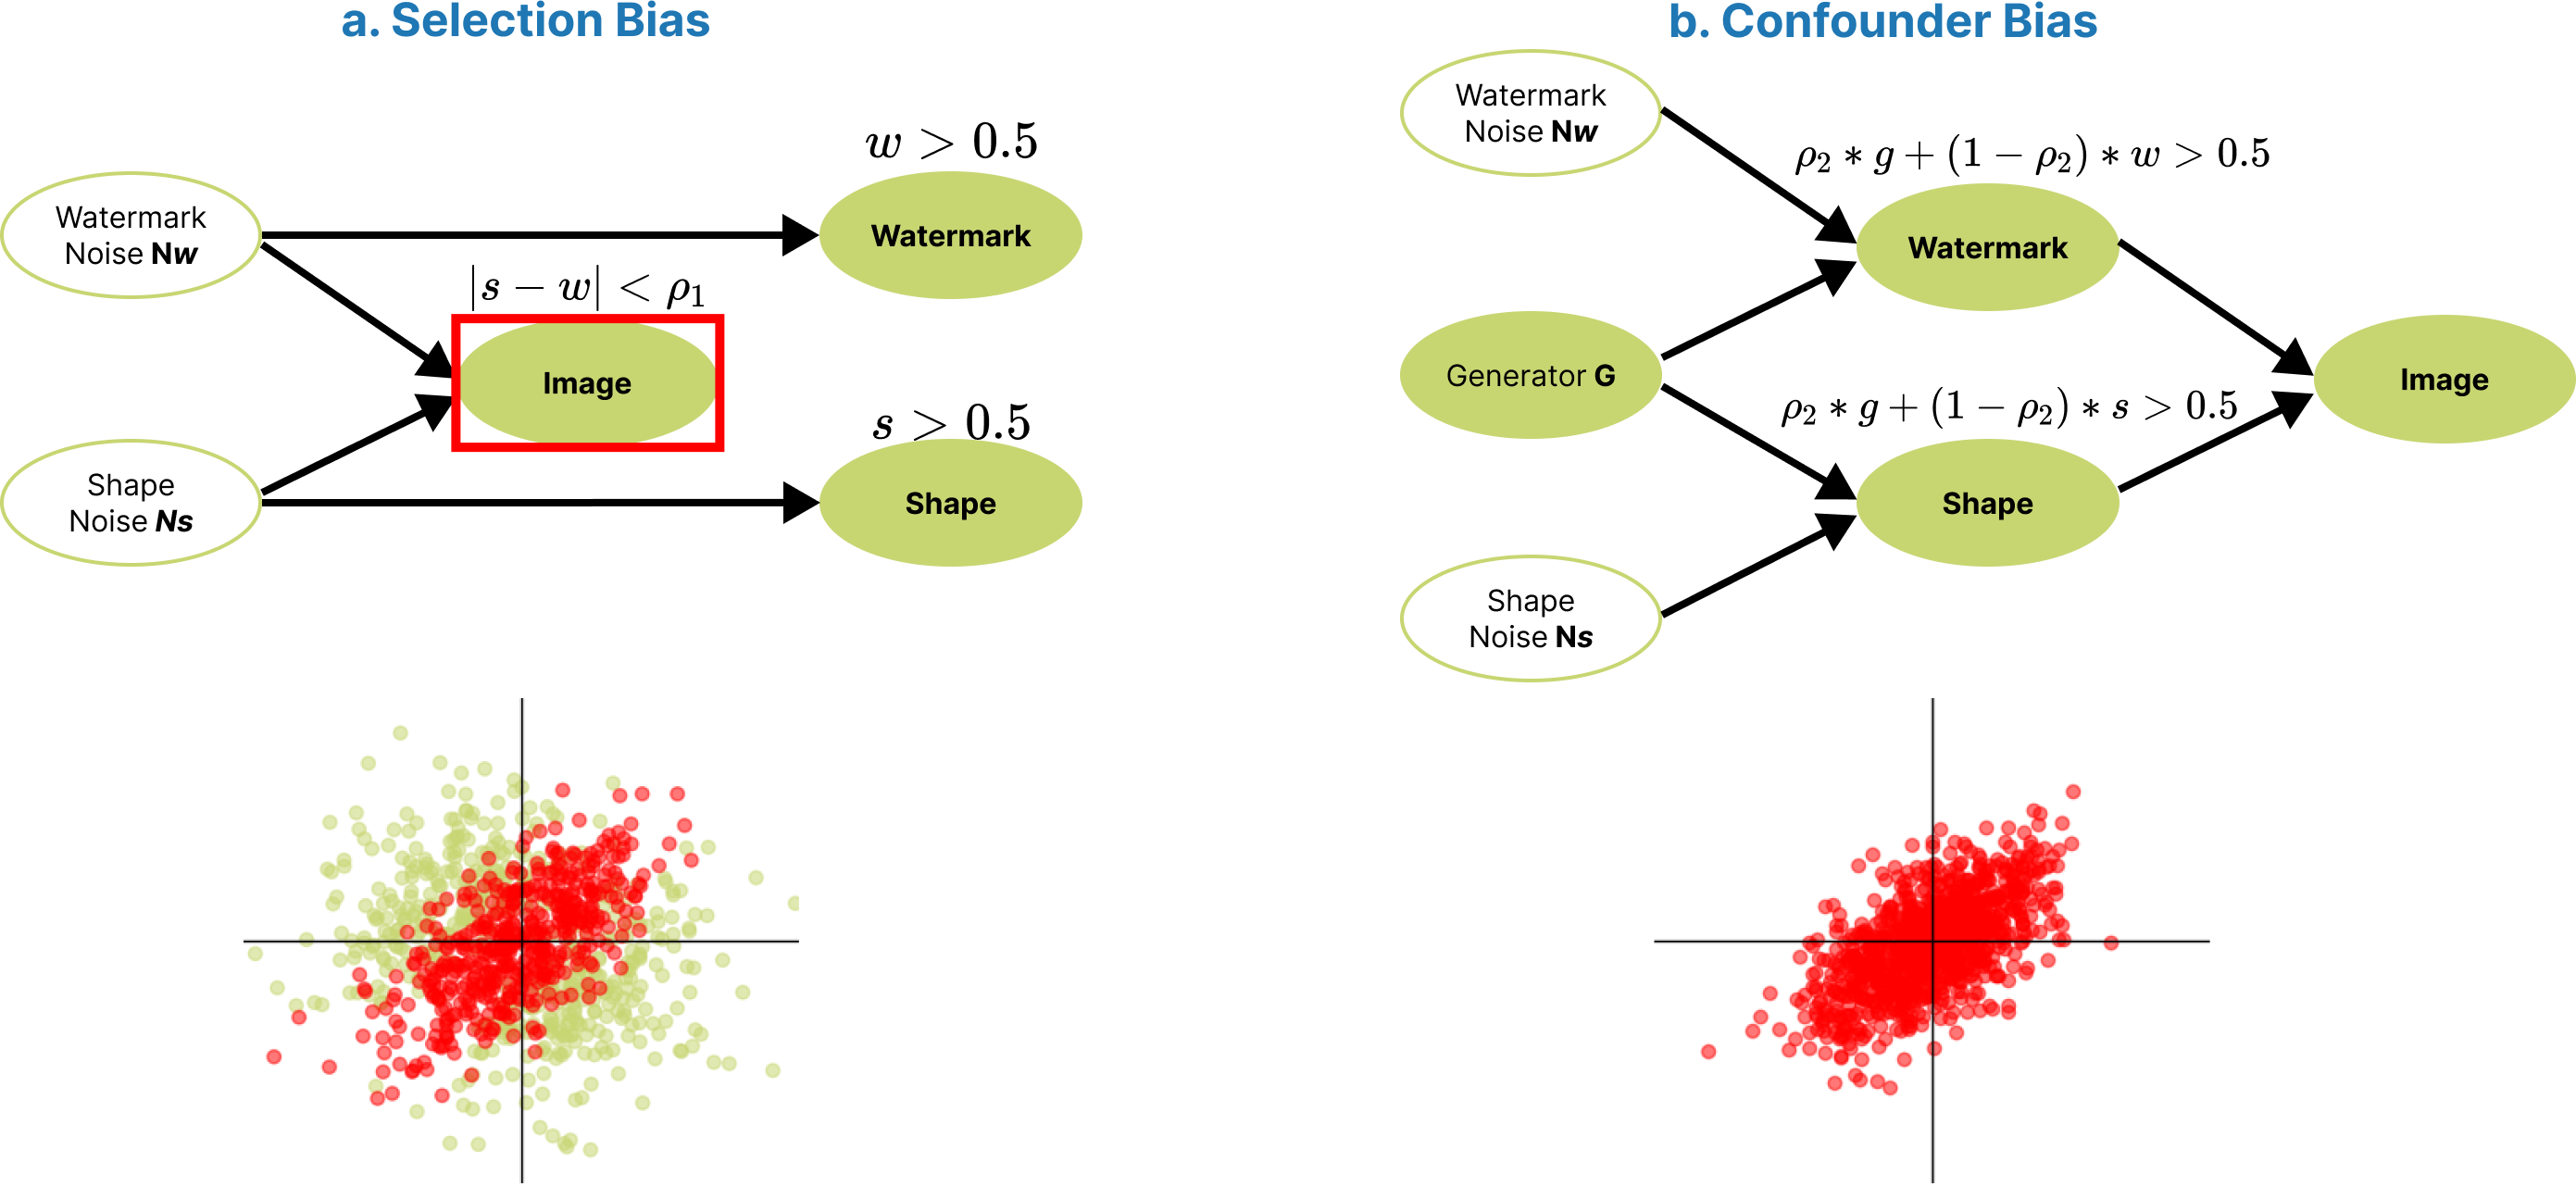
\includegraphics[width=0.8\textwidth]{pics/equivalent_scm.png}
    \caption[Selection and Confounder Bias]{SCMs typically found in image datasets.\\
    \textbf{a.} selection bias, e.g., ``researcher chooses horse images from free online collection with watermarks'': two generating variables are correlated because the image unintentionally is selected on in a particular way. \\
    \textbf{b.} confounder bias, e.g., ``photographer that uses watermark, mostly shoots horses'': a third variable (here the photographer) influences both variables. }
    \label{fig:equivalent_scm}
\end{figure}

It is important to note that this particular SCM is just one of many possible ways to model how spurious features might interact with target features. It attempts to follow the logic of how images are generated or selected in real datasets. Here, it particularly looks at pathways for the generation of Clever-Hans or watermark features, often present in image datasets \citep{Lapuschkin2019}. As visible in \cref{fig:equivalent_scm} different causal models can produce an equivalent distribution of the two latent factors in question (watermark and shape). One can think of more variations of SCMs which are able to produce the same correlation, so the choice of using the confounder version as in \cref{fig:generating_scm} is mainly due to its ease of implementation. It also lends itself best to the Clever-Hans task, because in this SCM there is no real causal effect between the target and spurious feature. It would therefore be ideal if a neural network would ignore the spurious feature completely. Without assumptions about the generating mechanisms though, the confounder case is not identifiable, or in other words, distinguishable from $W \rightarrow G \rightarrow S$ and $S \rightarrow G \rightarrow W$. 
Although the presented collider case (\cref{fig:equivalent_scm}\textbf{a}) is theoretically distinguishable from the confounder case (\textbf{b}), one can not hope that a network which only has access to the intervened on (selected) data will recover this. Neither can we hence expect the explanation to make such a distinction.

The idea of investigating the effect of a coupling ratio $\rho$ was inspired by \citet{Clark2023}, who also used a \textit{signal-to-noise} ratio in their generating model. Instead of a confounding model their learned data instances are colliders of the label and a suppressor variable similar to \cref{fig:equivalent_scm} \textbf{a}. In their experiments the expected explanation importance of a suppressor feature ought to be zero, as long as the collider is not intervened on, but also when the suppressor and target feature are coupled through smoothing of the image. We contest this assumption, as it is not clear whether a neural network does not implicitly condition on this collider (which is the image set), therefore introducing correlation between the parent components through a different kind of selection bias. We disagree with their statement that a good explanation method ought to not attribute any importance to such suppressor variables. This is, as  \citet{Nauta2023} put it, a case of conflating external \textit{coherence}, i.e., ``agreement with human rationales'' \citep{Atanasova2020} with \textit{correctness} towards the model. As we are not aware of any explicit way in which deep neural networks differentiate between a suppressor or confounder variable, it is unwarranted to expect an explanation to explain something the model does not even conceptualize. 

The direction of causal links for image classification is, as can be seen from this example, highly debatable and shall not be the focus of this work. Whether the selection of the AI researcher reducing costs with free images resulted in classes being polluted with watermarks (\cref{fig:equivalent_scm}\textbf{a}), or whether a scientist marked x-rays with their diagnosis (\cref{fig:equivalent_scm}\textbf{b}) seems to not be distinguishable for ML models. 
Instead, we only want to find to what degree a neural network learns and attribution method explains the distribution generated by a particular SCM.

\subsection{Explanation Generating Model}
The data generation causal model is part of the model which generates predictions and explanations.
This model is defined in a similar way to the \textit{explanation generating process (EGP)} by \citet{Karimi2023}.
Ratio $\rho$ is a meta-variable of our image generation process in a similar sense to how hyperparameters are defined for the training there. While \cref{fig:generating_scm} depicts the data generating causal model (DGCM) of the training dataset in more detail, \cref{fig:egp} shows how this is embedded into the mechanism of generating explanations. 

\begin{figure}[t!]
    \centering
    \tikzset{%
        neuron/.style={
            ellipse,
            draw,
            minimum height=8mm,
            },
        arrows={[scale=1.2]}
    }
%\begin{mdframed}[backgroundcolor=graybg]
    \begin{tikzpicture}[]
    % generating model:
        \node [neuron]  (r) at (0,4) {$\rho$};
        \node [neuron]  (rs) at (5,3) {seed};
        \node [neuron]  (scm) at (3,4) {DATA};
        \node [neuron]  (w) at (7,4) {weights};
        \node [neuron]  (x) at (7,2) {$X$};
        \node [neuron]  (p) at (9,3) {$Y$};
        \node [neuron]  (e) at (11,2) {$E$};
        
        \draw[->] (r) -- (scm);
        \draw[->] (scm) -- (w);
        \draw[->] (rs) -- (w);
        \draw[->] (w) -- (p);
        \draw[->] (x) -- (p);
        \draw[->, bend left=40] (w) to (e);
        \draw[->, bend right=20] (x) to (e);
        \draw[->] (p) -- (e);
    \end{tikzpicture}
%\end{mdframed}
    \caption[Explanation Generation Process (EGP)]{Explanation Generation Process: $\rho$ influences the data distribution, which together with the random initialization seed determines the weights of the model after training. The output $Y$ results from multiplying input samples $\mathrm{x} \in X$ with the weights. The explanation $E$ in turn depends on the output, the weights and the input sample.\textit{EGP}}
    \label{fig:egp}
\end{figure}

